%!TEX root = ../Dimensionieren I.tex

\section{Optimale Gesamtlösungen} % (fold)
	\begin{enumerate}
		\item Sicherheit gegen Versagen. (Bruch, Fliessen, Knicken, Beulen, zu grosse Deformationen, Ermüdung)
		\item Gleichmässige Beanspruchung
		\item Ökonomische Verbindung von 1. und 2.
	\end{enumerate}
% section: Optimale Gesamtlösungen (end)
\section{Rand-/Rahmenbedingungen} % (fold)
	\begin{tightitemize}
		\item Markt (Planung)
		\item Unternehmen
		\item Allgemeines Umfeld
		\item Technisches Umfeld
	\end{tightitemize}
% section: Rand-/Rahmenbedingungen (end)
\section{Entwicklungsprozess} % (fold)
	\begin{enumerate}
		\item Definitionsphase (System steht im Vordergrund)
			\begin{enumerate}
			\item Planung
			\item Konzept
			\item Vorentwicklung
			\end{enumerate}
		\item Realisierungsphase (Bauteil steht im Vordergrund)
			\begin{enumerate}
			\item Detailphase
			\item Prototyp
			\item Produktion
			\end{enumerate}
	\end{enumerate}
	
	\subsection{Konzeptphase} % (fold)
		\begin{tightitemize}
			\item Ausarbeiten der Anforderungsliste.
			\item Aufgliedern in Teilfunktionen.
			\item Erarbeiten von Lösungsansätzen.
			\item Erarbeiten von Konzeptvarianten.
			\item Bewertung der Varianten.
		\end{tightitemize}
	% subsection: Konzeptphase (end)
	\subsection{Vorentwicklungsphase} % (fold)
		Kritische Konstruktionsbereiche auf Realisierbarkeit prüfen.
		\begin{tightitemize}
			\item Ausarbeiten der Konstruktion
			\item Dimensionieren der Bauteile
			\item Detaillierung und Optimierung ausgewählter Bauteile
		\end{tightitemize}
	% subsection: Vorentwicklungsphase (end)
	\subsection{Detailphase} % (fold)
		\begin{tightitemize}
			\item Genaue Dimensionierung der einzelnen Komponenten.
			\item Prototyp-Evaluation
		\end{tightitemize}
	% subsection: Detailphase (end)
% section: Entwicklungsprozess (end)
\section{Ablauf einer Bauteildimensionierung} % (fold)
	\begin{enumerate}
		\item \textbf{Betriebszustände bestimmen}
			\begin{enumerate}
				\item Nenngrössen: Maximalwerte, die bei Normalbetrieb häufig auftreten.
				\item Nennspannungen: Für geg, Kräfte / Momente in definierten Querschnitten.
				\item Maximale Belastung (Abweichung von Nennbelastung):
				\begin{equation*}
					F_{\text{max}}=c_{\text{B}} \cdot F_{\text{Nenn}} \quad \text{mit} \quad c_{\text{B}} \text{: Betriebsfaktor}
				\end{equation*}
			\end{enumerate}
		\item \textbf{Kritische Bauteile auswählen}
			\begin{enumerate}
				\item Selektion durch Überlegungen: Kraftfluss, Kraftumlenkungen, Kraftverengungen.
				\item Gestalterische Optimierung.
			\end{enumerate}
		\item \textbf{Freilegen, Belastung bestimmen}
			Freischneiden und Einführen von äusseren Kräften/Momenten. Seile und Ketten: Zugkräfte. Stäbe: Zug-/Druckkräfte.
		\item \textbf{Kritische Bauteilquerschnitte und Schnittkräfte bestimmen}
			Kräfte- und Momentenverlauf einzeichnen. In Kombination mit Geometrie abschätzen.
		\item \textbf{Beanspruchung in kritischen Querschnitten}
			\begin{enumerate}
				\item Einfache Formen: Grobe Dimensionierung: Zug, Druck, Biegung, Torsion, Hertz'sche Pressung und Beanspruchung rotationssymmetrischer Körper.
				\item Komplexe Formen: Numerische Verfahren (FEM etc.)
				\item Prinzip von Saint Venant: Bei punktueller Krafteinleitung klingen innere Kräfte und Formänderungen ab, wenn man genug weit weg ist.
			\end{enumerate}
		\item \textbf{Festigkeits- und Versagenshypothesen}
			\begin{equation*}
				\sigma_{\text{zul}}=\frac{\sigma_{\text{G}}}{S_i}
			\end{equation*}
		\item \textbf{Ergebnisse diskutieren und optimieren}\\
			$\rightarrow$ Festigkeitsnachweis.
	\end{enumerate}
% section: Ablauf einer Bauteildimensionierung (end)
\section{Beanspruchungsarten} % (fold)
	\begin{tightitemize}
		\item Statische Beanspruchung
		\item Ermüdungsbeanspruchung $(\text{Lastspielzahl } N >10^4)$
	\end{tightitemize}
% section: Beanspruchungsarten (end)
\section{Bauteilversagen} % (fold)
	\begin{description}
		\item[Fliessen:] plastische Deformation
		\item[Bruch:] nach elastischem Verhalten\\
			% TODO: besseres Bruchbild
			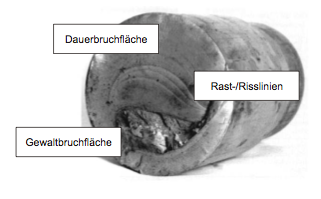
\includegraphics[width=0.6\columnwidth]{graphics/bruchbild}
		\item[Deformation:] eingeschränkte Geometrie (Funktion nicht mehr ge\-währ\-leistet)
		\item[Instabilität:] Knickung / Beulen
	\end{description}
% section: Bauteilversagen (end)
\section{Werkstoffkennwerte} % (fold)
	\begin{tightitemize}
		\item Grenzwerte ( Proportionalitäts-, Fliess-, Streck-, Dehngrenze etc.)
		\item Temperatureinfluss
	\end{tightitemize}
% section: Werkstoffkennwerte (end)
\section{Sicherheitsfaktoren} % (fold)
	Die Sicherheitsfaktoren spielen folgende Rolle:
	\begin{tightitemize}
		\item Unsicherheiten
		\item Werkstoffkennwerte
		\item Fertigungstoleranzen
		\item Berechnungsmethoden
	\end{tightitemize}
% section: Sicherheitsfaktoren (end)
\section{Normierung für Belastungen} % (fold)
	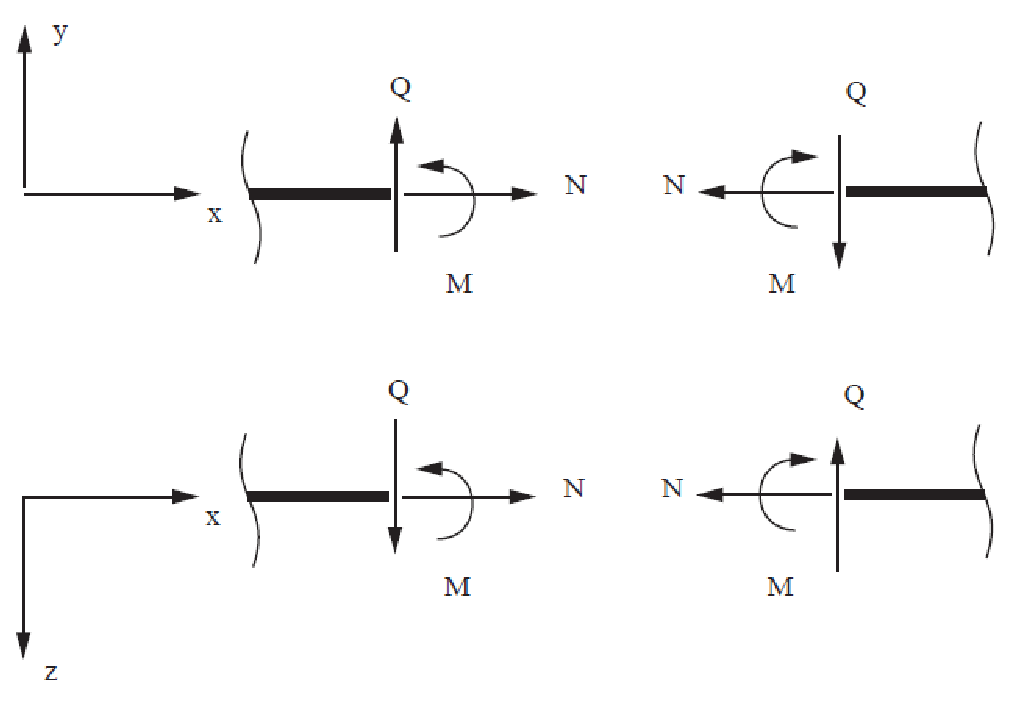
\includegraphics[width=\columnwidth]{graphics/belastungen}
% section: Normierung für Belastungen (end)